\documentclass[runningheads]{llncs}
\usepackage[latin9]{inputenc}
\usepackage{url}[obeyspaces]
\usepackage{amsmath}
\usepackage{alltt}
\usepackage{graphicx}
\usepackage[unicode=true,
 bookmarks=false,
 breaklinks=false,pdfborder={0 0 1},backref=section,colorlinks=false]
 {hyperref}

\makeatletter
%%%%%%%%%%%%%%%%%%%%%%%%%%%%%% User specified LaTeX commands.
% This is samplepaper.tex, a sample chapter demonstrating the
% LLNCS macro package for Springer Computer Science proceedings;
% Version 2.20 of 2017/10/04
%
% Used for displaying a sample figure. If possible, figure files should
% be included in EPS format.
%
% If you use the hyperref package, please uncomment the following line
% to display URLs in blue roman font according to Springer's eBook style:
% \renewcommand\UrlFont{\color{blue}\rmfamily}





% SJT use this to get nicer formatting of textual identifiers in math mode
\newcommand{\ident}[1]{\mbox{\emph{#1}}}


\usepackage{listings}
\renewcommand{\lstlistingname}{Listing}



\usepackage{listings}
\renewcommand{\lstlistingname}{Listing}





\usepackage{listings}
\renewcommand{\lstlistingname}{Listing}



\makeatother

\usepackage{listings}
\renewcommand{\lstlistingname}{Listing}

\begin{document}
\title{Standardized crypto-loans on\\ the Cardano blockchain}%\thanks{Supported by Cardano Foundation.}}


\author{Dmytro Kondratiuk\inst{1}\orcidID{XXXX} \and
				Pablo {Lamela Seijas}\inst{1}\orcidID{0000-0002-1730-1219} \and
                Simon Thompson\inst{1,2}\orcidID{0000-0002-2350-301X}}

\authorrunning{D. Kondratiuk, et al.}

\institute{IOHK, Hong Kong,
\email{dmytro.kondratiuk@iohk.io, pablo.lamela@iohk.io, simon.thompson@iohk.io}  \and
School of Computing, University of Kent, UK,
\email{s.j.thompson@kent.ac.uk}}



%
\maketitle              % typeset the header of the contribution
%
\begin{abstract}
Crypto-loans are %unique and 
innovative financial instruments that
allow trustless peer-to-peer %P2P 
lending, and potentially providing a safe and convenient
source of liquidity for cryptocurrency holders. In this paper we
explore a smart contract framework for building standardized crypto-loans
using the Marlowe domain-specific language and with the ACTUS standard at its core.

\keywords{ACTUS \and blockchain \and Cardano \and finance \and Haskell \and Marlowe} 
\end{abstract}


\textbf{DONE:}
\begin{enumerate}
\item
Added overview at the end of the intro.
\item
Tidying up identifiers in math equations using the command \verb+\ident{...}+
\item
Biblio sorted out ordering (added keys). shortened author and editor lists
\item
Revised sections 2--7.
\end{enumerate}

\textbf{TO DO:}
\begin{enumerate}
\item
Deal with inline comments in source code: \verb+% SJT ...+
\item
Write introduction [SJT]
\item
Should we include Alex as co-author?
\item
What about R (shiny)?
\item
We use \verb+equation+ environment which numbers equations, but the numbering isn't used I think.
So I'd suggest moving to \verb+equation*+ instead (easy edit).
\end{enumerate}


\section{Introduction}



\bigskip\noindent
List of contributions:
\begin{itemize}
\item \textquotedblleft Marlowe Labs\textquotedblright{} editor on Playground
(Dmytro) 
\item R Shiny cashflow visualiser for ACTUS (Dmytro) 
\item ACTUS Utility functions (Dmytro, Quanterall) 
\item executable ACTUS spec for PAM (Dmytro, Alex) 
\item executable ACTUS spec for LAM (Wyo Hackathon) 
\item Library for generating ACTUS contracts (Dmytro) 
\item ACTUS-like examples on Playground (Dmytro, Alex, Pablo) 
\item Marlowe DSL enhancements for Actus: Cond, Mul (Dmytro) (draft) 
\item ACTUS spec generator for Agda (Dmytro) 
\item Auto-refund static analysis (Pablo) (partial: only QC) 
\item Verification with QC + SMT (Dmytro) 
\end{itemize}

A note on notation: \texttt{typewriter} font will be used for Marlowe constructs
% SJT and fragments?
while \emph{math} font will be used for mathematical formulas and pseudo-code.
% Have I got this right?
% dk14 looks right to me - I didn't know how to highlight Marlowe constructs properly

% SJT: added this overview of the paper
% it is traditional to end the introduction like this,
% 'signposting' what is in the rest of the paper.
Section \ref{background} of the paper covers the relevant financial background, and Section \ref{modelling} introduces Marlowe as well as the ACTUS financial standard. Section \ref{executable} builds an executable specification of ACTUS in Haskell, and this is used in Section \ref{generation} to generate  the Marlowe code for an ACTUS contract from the terms of the contract. Section \ref{tokenization} explains how tokens are used to represent ownership of roles in a running contract, and Section \ref{assurance} describes how we provide assurance that  contracts behave as they should. Section \ref{related} examines related work and Section \ref{conclusion} concludes. 



\section{Financial contracts}
\label{background}

A loan is a form of debt incurred by an individual or other entity.
The lender advances a sum of money to the borrower. In return, the
borrower agrees to a certain set of terms including any finance charges,
interest, repayment date, and other conditions \cite{loan}.

Cryptocurrency-backed loans must have \emph{collateral} when there is no trust
between party and counterparty. While a loan is usually settled in a
stable-coin currency (e.g. USDT/USDC), collateral is typically denominated
in a cryptocurrency (e.g. BTC). The purpose of such a loan is to give
the borrower access to the fiat value of their crypto-funds without
actually selling them for fiat. The borrower pays interest in exchange
for gaining liquidity.

Every loan has a positive net payoff (return minus investment) that
is either rendered as a one-time payment -- often called a \emph{zero-coupon bond} (ZCB) -- or by scheduling
payment of the interest. The rate of interest could be fixed throughout
the lifetime of a contract: for example, zero-risk bonds have a fixed
interest proportional to the inflation rate.
However, in the generic case the interest rate is variable and depends
on an external factor agreed in advance, and the rate is periodically
updated by observing the state of that factor. 

Such loans often represent an investment in a particular venture or industry. As
a somewhat fictional example, one could imagine a cryptocurrency miner
who decided to scale their crypto-farm: a loan (in USD) with variable
interest that directly depends on cryptocurrency prices would be more
attractive for a miner because it would directly correlate with miner's
profits. For example, if the price of the cryptocurrency goes down
in a particular month the borrower would have to pay lower interest, and so would always pay a fixed share of the profits. In a more traditional
setup the interest rate could depend on prices of other commodities: the canonical example would be a power plant taking a loan
with interest depending on electricity prices. 

In both cases, the prices of
cryptocurrency or electricity become a driver for the interest
rate.
However, one cannot simply take the bare price of the asset and turn
it into a rate. In order to make \emph{units of measurement} compatible
%SJT compatible with what??
adjustments should be made. Fluctuations of the interest rate driver
are embedded thus:

% SJT a couple of questions about these equations
% Q1
% What is the role of the subscript r in \Delta_r
% Q2
% interest rate at t+1 defined from rate at t-1. I'd have expected just one difference, so
% t+1 defined from t, or t defined from t-1.

% dk14 
% A1 it is from the ACTUS spec - I assume "r" means "rate"
% A2 I meant "before vs after event", but I'll remove it

\noindent 
\begin{equation*}
\Delta_{r}=\ident{capfloor}(\ident{driver}*\ident{multiplier}+\ident{spread}-\ident{interestRate}_{t-1})
\end{equation*}

\noindent 
\begin{equation*}
\ident{interestRate}_{t}=\ident{capfloor}(\ident{interestRate}_{t-1}+\Delta_{r}),
\end{equation*}

\noindent
where \emph{capfloor} is a function that limits the range of fluctuation,  
and so limiting the lender's exposure to risk:

\noindent 
\begin{equation*}
\ident{capfloor}(x)=\ident{max(min}(x,\ident{floor}),\ident{cap})
\end{equation*}

\noindent
The \emph{spread} parameter here loosely represents the difference between
the average prime 
% SJT explain "prime" here.
% it's standard financial terminology: https://www.investopedia.com/terms/p/primerate.asp
rate that the lender expects -- the \emph{benchmark yield} -- and
the rate imposed by the driver - the higher the spread, the higher
the resulting interest rate. The multiplier %effectively 
rescales the interest rate value 
% SJT used value here rather than plot: is that OK?
% dk14 maybe "curve" would be better
in order to represent the changes to be made converting between different units
of measurement: how many rate percentage points 
% SJT percentage points of what?
% dk14 rate
you would get for a USD-to-kilowatt conversion
and so on.

In the context of ACTUS and simillar frameworks, 
% SJT - need to explain "event-based" in this context.
% dk14. "Event-driven" but it has no relation to scaling, so I'll remove it
there is
one more factor influencing interest rates thorough scaling:

\noindent 
\begin{equation*}
interestPayment=interestScalingFactor*interestRate*notional
\end{equation*}
\noindent
This scaling is dynamic and loosely adjusts for variance (volatility)
of the asset that the interest rate driver represents.

\paragraph*{Interest accrual and capitalisation. }

A counterparty might decide to reinvest profit received as interest
from the %same 
% SJT I think "same" is superfluous here: is that OK?
% dk14 sure
loan. In the simplest case, this renders as compound
interest. This can be modelled through interest accrual and capitalisation;
% SJT what does "capitalisation" mean?
% dk14 "conversion of income or assets into capital" it's quite googlable financial terms so idk if I should note it explicitly
for instance, contracts from the ACTUS specification accrue interest
between interest payments and can transfer interest to a notional
during interest capitalisation event (IPCL).

Overall, variable interest rates introduce a certain risk for a lender,
thus they can be %are 
subject to hedging. While any instrument that depends
on the same risk factor (interest rate driver) would suffice, the
most popular way to hedge a variable interest rate loan is an interest
rate swap. This instrument allows two (or more) parties to exchange
their incomes - one from a fixed interest rate loan, the other from a variable-rate loan.

\paragraph*{Counterparty risk.}

Trustless setups, especially ones in the cryptocurrency world, including 
decentralised smart-contracts and exchanges, require no trust between
party and counterparty involved in a contract. In case of a loan,
this literally means that counterparty has zero obligation to pay
the money back, thus rendering the loan useless for a party. Such
risks are usually addressed by introducing collaterals, as in the following scenario. 
\begin{enumerate}
\item Alice would like to borrow 1000 USD 
\item She has Bitcoin assets cost around 1500 USD, which she intends to
hold throughout a year, so Alice has high confidence in the market
(she expects prices to double or triple) 
\item Bob would like to lend 1000 USD and get an interest higher than traditional
interest rate offered by banks (let's say 15\% instead of 10\%). He
is either bearish or neutral towards Bitcoin. 
\item Alice transfers her BTC as collateral to a contract, and Bob transfers
his USD to Alice 
\item If Alice pays the interest and notional on time, and the BTC price does not
render collateral worthless, she can get her collateral back; otherwise
the loan gets liquidated and the collateral is transferred to Bob. 
\end{enumerate}

\section{Modelling financial contracts}
\label{modelling}

This section introduces the Marlowe domain-specific language (DSL) and the ACTUS standard for financial contracts.

\subsection{Marlowe}

Marlowe~\cite{marlowe} is a high-level DSL for writing
financial contracts on blockchain. Marlowe is defined
by an executable semantics in Haskell, and has been implemented on
the UTxO-based Cardano blockchain. 
% SJT added this
%dk14 OK
Marlowe contracts are finite, and moreover have defined finite lifetime. This means that it is possible to perform \emph{static analysis} on them. For example, it is possible symbolically to check \emph{all} execution paths without running a contract, and in particular checking that every \texttt{Pay} construct can be executed in full.

The main advantage of using Marlowe to carry ACTUS logic is enhanced
security that such a static analysis provides. SMT-solvers~\cite{smt} are gaining
popularity as an alternative to fuzzing when it comes to testing software
for vulnerabilities. Smart contracts generated from ACTUS
specification are quite complicated, so manually testing every possible
execution path for every possible combination of contract terms is
not feasible. Static analysis, in turn, can reduce the amount of ``dumb''
mistakes that could cost millions to the users by ensuring obvious
properties of a contract. It is not a panacea, however, unlike with
fuzzing, if SA says that certain property holds - it does it with
100\% assurance.

\subsection{ACTUS}
\label{ACTUS}

The Algorithmic Contract Types Unified Standards (ACTUS)~\cite{actus} define the logic embedded in legal agreements that eventually
turn the contract terms into actual cash flows, or more generally
business events. Most of its basic contract types represent
different variations of lending contracts.

ACTUS relies on a state machine formalism in order to describe the
behaviour of a given contract. Every \emph{payoff} -- i.e. transfer of funds in
or out of a contract -- can be inferred for any given state. Every state
can be derived from previous events and observed risk factors:

\noindent 
\begin{equation*}
\ident{payoff}_{i}=\ident{POF}(\ident{state}_{i})
\end{equation*}

\newcommand{\STF}{\ident{STF}}
\noindent 
\begin{equation*}
\ident{path}=\STF_{1}(ct,ev_{1})\circ \STF_{2}(ct,ev_{2}).\circ\ldots\circ \STF_{i}(ct,ev_{n})
\end{equation*}

\noindent 
\begin{equation*}
\ident{state}_{i}=\ident{path}(\ident{INIT}(ct)),
\end{equation*}
\noindent
where \emph{ct} stands for contract terms, \emph{INIT} returns initial state, \emph{sched}
returns scheduled events, \emph{STF} takes \emph{contractterms}, \emph{event}, and \emph{state}
and returns the next state, and \emph{POF} returns the payoff in a state.

\subsection{Oracles}

In order to support variable interest rates and scaling, ACTUS requires
a smart contract to be able to observe the value of a given risk factor,
such as an interest rate, at a particular point in time $t$. This is due to the state of the risk factor not being known at instantiation
time. 

% SJT - the "i" and "t" subscripts here look a bit odd: is that what's intended?
% dk14 - fixed
\noindent 
\begin{equation*}
\ident{riskfactor}_{it}=O_{\footnotesize\ident{rf}}(i,t)
\end{equation*}
\noindent
In the case of the Cardano blockchain, these values are usually
provided through an \emph{oracle} mechanism\cite{oracles}. An oracle
could be a trusted party providing necessary data or network of parties
under consensus \cite{de-oracles}. 
% SJT REF needed
% dk14. I've found this one has explanation for oracles (ChainLink etc)

From a Marlowe DSL perspective,
the exact mechanism that provides external data is less important,
as Marlowe abstracts over IO by requiring a particular type of input -- a 
\texttt{Choice} -- that is protected with a cryptographic signature by the source of the choice.
% SJT changed from "owner" to "source".
% dk14 OK
As a result, the event of receiving data from an oracle is treated the
same as receiving numeric input in other languages

\section{Building an executable specification of ACTUS}
\label{executable}

ACTUS is defined in a textual specification\footnote{Available from \url{https://www.actusfrf.org/techspecs}.} which, while expressed in mathematical notation, is essentially informal. In this section we describe how this specification is turned into an \emph{executable} version by rendering it in Haskell. This translation is in fact a transliteration, since notation, variable names and so forth are respected.
% SJT: are you happy with this? If not, let's rephrase,
% but it would be good include something to this effect.
% dk14 thanks for adding this

\subsection{Rendering the specification in Haskell}

The ACTUS standard is specified in terms of scheduling, payoff and
state transition functions that are polymorphic on event and contract
type, as noted in Section \ref{ACTUS} above. The specification also follows quite specific naming conventions
that are incompatible with Haskell's conventions. The executable specification
follows original ACTUS conventions as closely as possible in order to
ease code base maintenance when faced with updates of the ACTUS
spec repository\footnote{\url{https://github.com/actusfrf/actus-techspecs}}.

Using Haskell itself as a DSL for explicitly encoding formulas without
using advanced language idioms also simplifies code generation. 
In case of ACTUS this comes at a cost reduced type-safety, handling nullable
values explicitly introduces risk of exceptions. However this risk
is addressed using property-based testing, and in particular QuickCheck generators. This is discussed in more detail in Section \ref{verification} below.
% SJT Added x-ref to section 7.

\subsection{Utilizing polymorphism to abstract over basic operations}

In order to keep our executable specification independent of the carrier -- whether it is a smart-contract engine, proof assistant, analytical framework
or even machine learning model -- we abstract over the underlying representation
of state variables,

\begin{verbatim}
-- Definitions/ContractState.hs 
data ContractStatePoly a b = ContractStatePoly  
{  
  tmd     :: b  
  , nt    :: a  
  , ipnr  :: a  
  , ipac  :: a  
  , feac  :: a  
  , fac   :: a  
  , nsc   :: a  
  , isc   :: a  
  , prf   :: ContractStatus  
  , sd    :: b  
  , prnxt :: a  
  , ipcb  :: a  
} deriving (Show) 
\end{verbatim}
\noindent
and arithmetic operations,
\begin{verbatim}
-- Ops.hs
class ActusOps a where    
   _min :: a -> a -> a
   _max :: a -> a -> a
   _zero :: a
   _one :: a

class ActusNum a where
   (+) :: a -> a -> a
   (-) :: a -> a -> a
   (*) :: a -> a -> a
   (/) :: a -> a -> a

class YearFractionOps a b where
   _y :: DCC -> a -> a -> a -> b   

class DateOps a b where
   _lt :: a -> a -> b --returns pseudo-boolean   

class RoleSignOps a where
   _r :: ContractRole -> a
\end{verbatim}
\noindent
Thus, every formula in the executable spec could be instantiated
to: 
\begin{itemize}
\item a formula on some \emph{atomic} type, like \texttt{Double} or \texttt{Day}, which could be used
to directly compute cash-flows for analytical purposes or precompute
payoffs for smart contracts that do not depend on oracles; or 
\item a formula representing a piece of \emph{abstract syntax}, e.g. a Marlowe \texttt{Value} or \texttt{Observation}, that could
be used to generate smart contracts that depend on oracles or to generate
code in another language, such as Agda.
\end{itemize}
This approach of abstracting formulas has a limitation of not allowing
conditionals to be expressed in an abstract way: in other words, there is no \texttt{ActusIf}
typeclass. Luckily most of conditional expressions in ACTUS specification
don't depend on variable state of a contract, they depend on \texttt{ContractTerms}
that are known in advance during contract generation. This allows
us to dispatch appropriate formulas during generation rather than
execution.

The only exception to this are the rare situations where we need to compare
2 state variables and choose either $\ident{formula}^\prime$ or 0 depending on the result of the comparison
result:

\begin{equation*}
\ident{formula}(st)=\begin{cases}
\ident{formula}^\prime(st) & \ident{var}_1(st)<\ident{var}_2(st)\\
0 & \ident{otherwise}
\end{cases}
\end{equation*}
We rely on a pseudo-Boolean \emph{less than} function in order to address
that:

\noindent 
\begin{equation*}
\ident{formula}(st)=\ident{pseudoLt}(\ident{var}_1(st),\ident{var}_2(st)))*\ident{formula}^\prime
\end{equation*}

\noindent 
\begin{equation*}
\ident{pseudoLt}(a,b)=\ident{Cond}(a>b,1,0)
\end{equation*}


\subsection{Contract term representation and explicit applicability}

In order to simplify serialisation and deserialisation of contract terms
across ACTUS related services maintained by Cardano we rely on ``superposed''
representation of contract terms: all ACTUS contract types are represented
with the same type. 

While such a representation allows both encoder
and decoder to express any ACTUS contract terms, it also allows for
invalid combinations of terms (for example \emph{PRNXT} cannot be applied
to a PAM contract), which means contracts require specific validation
that is implemented by means of the applicability function:

% SJT - do you mean \mapsto or \rightarrow here?
% dk14 - it is a mapping, but could be function/morphism too
\noindent 
\begin{equation*}
\ident{Applicability}:\ident{ContractTerms}\rightarrow \ident{Bool}
\end{equation*}

ACTUS standard defines a family of applicability functions polymorphic on contract
type:
% SJT something needed here.
% dk14 - we already gave a link to actusfrf, so I think I can skip references

\smallskip
% SJT changed ContractTerm to ContractTerms
% dk14 OK
\noindent 
\begin{equation*}
\ident{Applicability} : \ident{ContractType} \times \ident{ContractTerms} \rightarrow \ident{ApplicabilityType}
\end{equation*}
\noindent
where applicability could be: \emph{none}, \emph{always}, \emph{nullable}, or \emph{multiple}.

In order to build superposed contract terms type for such functions,
we have to resolve conflicting applicability types for merged contract terms
using the following resolution rules:

\noindent 
\begin{equation*}
\ident{weaken}(a_{1},a_{2})=\begin{cases}
\ident{nullable} & a_{1}=\ident{none}\wedge a_{2}=\ident{always}\\
\ident{nullable} & a_{1}=\ident{always}\wedge a_{2}=\ident{none}\\
a_{1} & \ident{priority}(a_{1})>\ident{priority}(a_{2})\\
a_{2} & \ident{otherwise}
\end{cases}
\end{equation*}

\noindent 
\begin{equation*}
\ident{priority}(x)=\begin{cases}
0 & x=\ident{always}\\
1 & x=\ident{none}\\
2 & x=\ident{nullable}\\
3 & x=\ident{multiple}
\end{cases}
\end{equation*}
\noindent
where $a_{i}$ is the applicability of a given term of the \emph{i}th contract
type to be merged.

\section{Generating Marlowe contracts from standardised ACTUS contract terms}
\label{generation}

In this section we describe how concrete Marlowe contracts are generate from the terms -- i.e. parameters -- of standard ACTUS contracts; we also describe the implementation of the system, and reflect on the limitations of generating contracts in Marlowe, where contracts have a a predefined lifetime and collection of interactions with contract participants.

\subsection{Overall architecture }

\begin{figure}
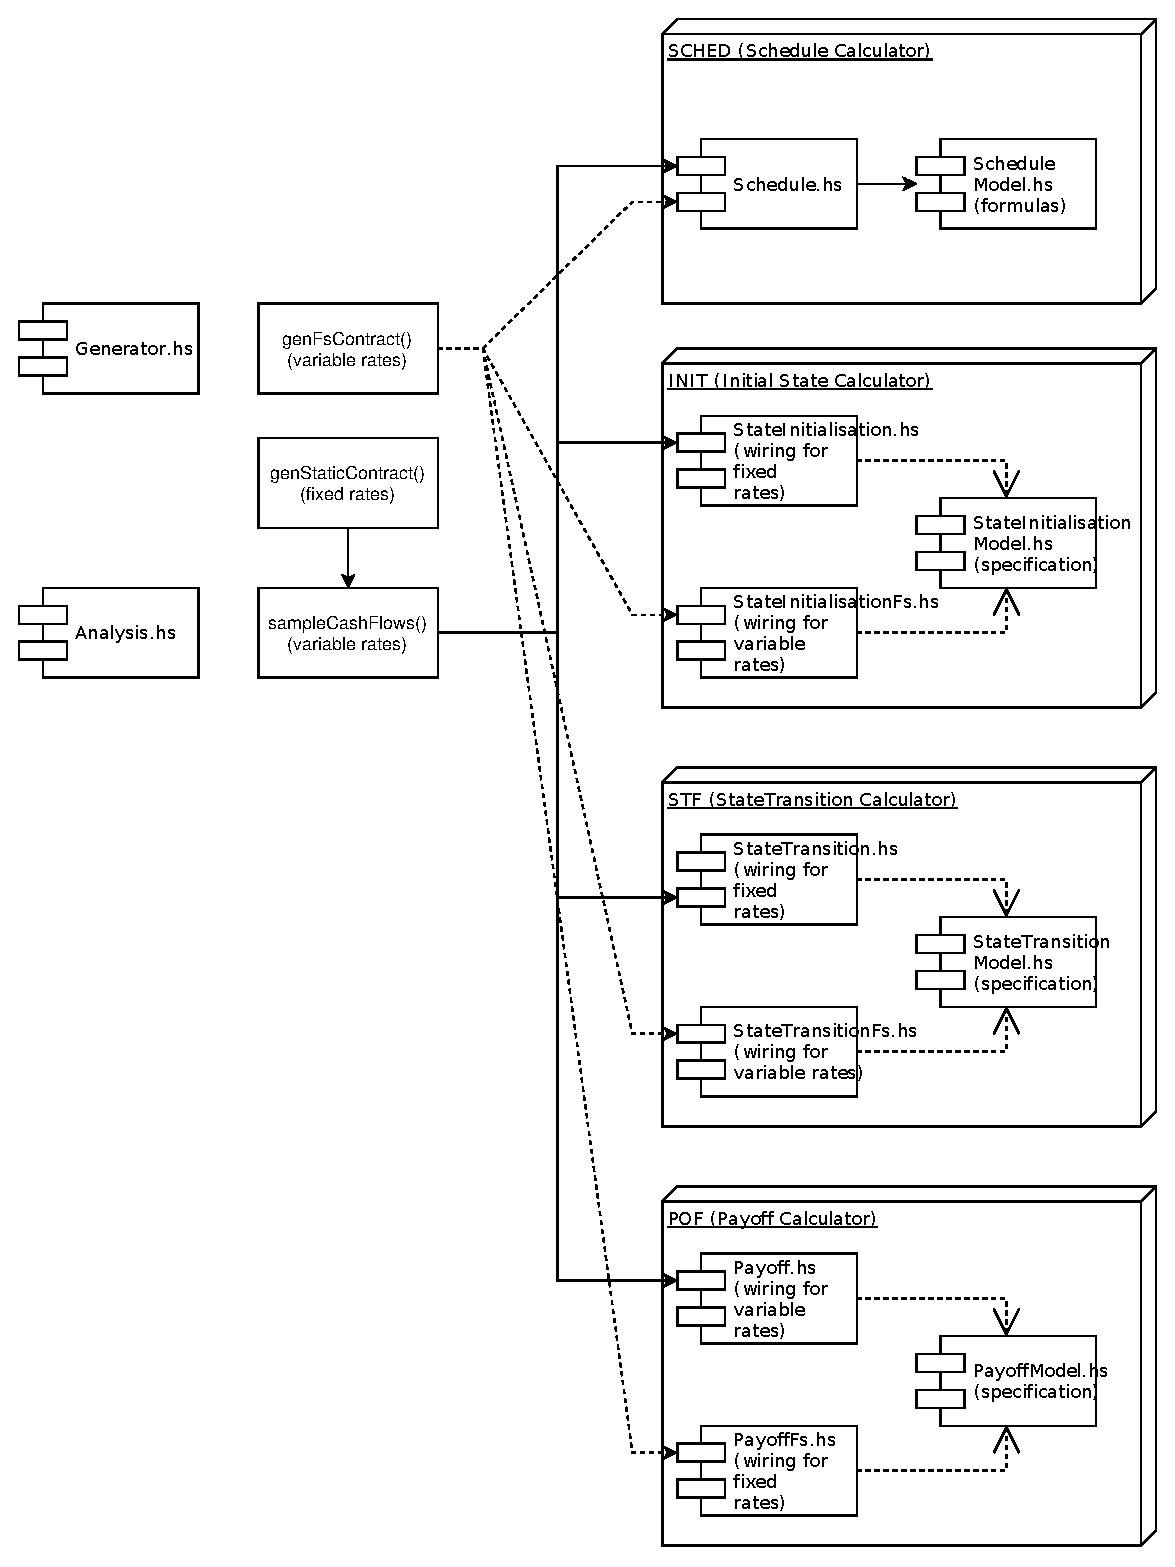
\includegraphics[width=1\textwidth]{images/modules} \caption{Modules responsible for contract generation.}
\label{fig1} 
\end{figure}

A generated contract is essentially a continuation chain of smaller contracts:

\noindent 
\begin{equation*}
\ident{chainlink}(t)=\ident{receiveData}(t)\circ \ident{calculatePayoff(t)}\circ \ident{processPayoff(t)}
\end{equation*}

\noindent 
\begin{equation*}
\ident{contract}(ct)=\ident{collaterals}(ct)\circ \ident{INIT}(ct)\circ\prod_{\footnotesize t\in \ident{SCHED(ct)}}\ident{chainlink(t)}
\end{equation*}

\noindent
where the component \emph{receiveData} asks an oracle for Marlowe Choice if needed, and
\mbox{\emph{calculatePayoff}} calculates the payoff formula. For fixed-rate contracts
this is optimised into a pre-calculated constant function. The \emph{processPayoff} function
awaits the \texttt{Deposit} of a payoff amount from a party: if the deposit is made them 
it directs the funds to a counterparty, otherwise it transfers
the collateral to the counterparty and closes the contract. The principal components of the system are shown in Figure \ref{fig1}. There are 3 categories of components representing ACTUS functions: specification with formulas, formula wiring for fixed rates (produces precomputed payoffs) and formula wiring for variable rates (produces Marlowe-code that computes payoffs). Different types of wiring correspond to different implementations of \emph{ActusOps} implemetations (either \emph{Double} or \emph{Value}). 
% SJT added this figure ref: OK?
% Do we need to add a little more to explain Fig1?
% dk14 OK, added few sentences about Fig1

The chain
is generated from the fixed schedule of events, known in advance of execution, 
using the \ident{SCHED()} function from ACTUS, as shown in Figure \ref{fig2}.
% SJT added this figure ref: OK?
% dk14 OK

\begin{figure}
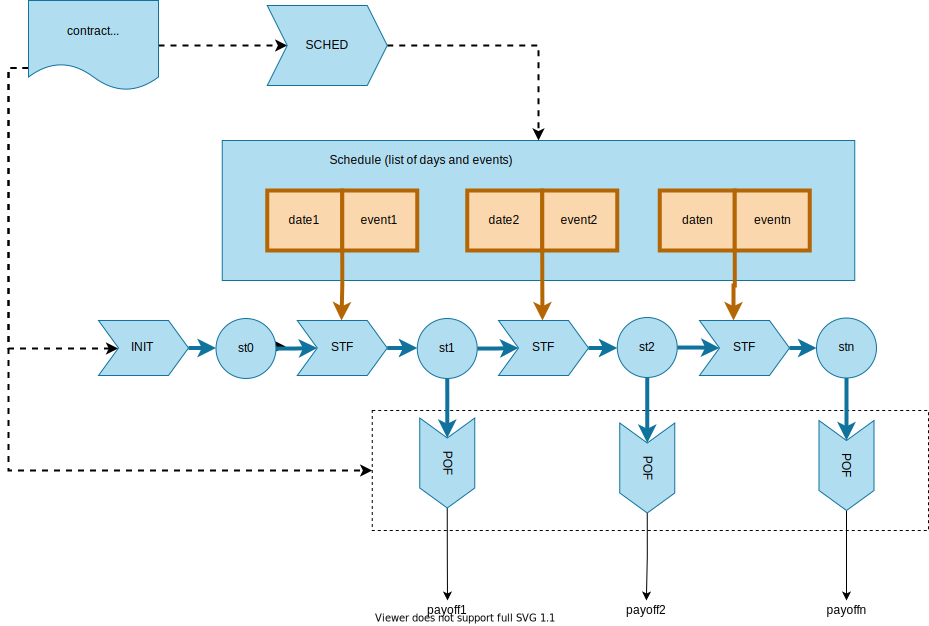
\includegraphics[width=1\textwidth]{images/flowchart} \caption{Chain of sub-contracts representing ACTUS logic}
\label{fig2} 
\end{figure}


\subsection{Avoiding exponential growth }

Marlowe contracts are finite, and in particular Marlowe itself does not have constructs for functions or recursion; these \emph{are} available in the Haskell and JavaScript embeddings of Marlowe, but they are unrolled on translation to pure Marlowe. Naive usage of the \texttt{If} operator in Marlowe could lead to exponential growth of a contract, as in this pesudocode example:

\begin{alltt}
if condition 
  then 
    perform\_something1()
    continue() 
  else 
    perform\_something2() 
    continue()
\end{alltt}
\noindent
Translating this to Marlowe would inline contents of \texttt{continue()} twice and, given that ACTUS
contracts are essentially generated using continuation as an accumulator,
this would lead to exponential explosion of the size of any ACTUS
contract that has conditionals in their state transition logic.

An example of such logic would be cap/floor limitations on interest rates:

\noindent 
\begin{equation*}
\ident{adjusted}=\ident{max(min(original,floor),cap)}
\end{equation*}
\noindent
We addressed this issue by introducing the \texttt{Cond} expression construct in order
to represent conditional expressions, rather than only conditional contracts as was the case before. Instead of using the \texttt{If}
contract to decide the value of some variable, we use a conditional expression instead.  
\texttt{Cond} is  a pure function
that returns a value depending on a condition, in contrast to the \texttt{If}
contract that chooses between two continuation contracts. 
% SJT I don't think we need to say this.
%The name is borrowed from a similar function in Lisp.
% dk14 - Oh sure. I was going to remove it too :)

\subsection{Limitations due to termination}

Marlowe doesn't allow contracts that run indefinitely, even if their recursion
is productive, as would be the case in a perpetual swap contract, for example. We therefore cannot support certain
contract types from ACTUS specification, namely the ones that don't
have a defined maturity date (like UMP). 

% In a long-term perspective
There is a possible workaround: contracts with no maturity date
could be represented as actors with a finite number of state transitions.
% SJT is this ^^^ rephrasing OK?
% dk14 - sure
We prototyped this approach, % in a separate branch, 
however it does
seem more prone to errors comparing to rendering predefined schedules.
More importantly, it greatly affects static analysis because the number
of reduction steps in the contract grows from 
\noindent 
\begin{equation*}
N_{\footnotesize \ident{scheduled}}=\ident{count(event)}
\end{equation*}
to 
\noindent 
\begin{equation*}
N_{\footnotesize \ident{stateTransitions}}=\frac{\ident{max(date(event))}-\ident{min(date(event))}}{\ident{precision}} 
\end{equation*}

\subsection{Fixed-point precision }

For numeric types Marlowe supports Integers, while ACTUS is expressed in terms
of real numbers. In order to model a real number in such a setup
we rely on fixed-point precision. The algebra looks like this: 
\begin{verbatim}
  (+)   = AddValue -- x/n + y/n = (x + y)/n
  (-)   = SubValue -- x/n - y/n = (x - y)/n
  a * b = Scale (1 % marloweFixedPoint) $ MulValue a b 
                            -- x/n * y/n = (x * y)/n^2
\end{verbatim}
We scale all numbers with \emph{marloweFixedPoint} factor - which only requires modification of \emph{MulValue}.
% SJT this needs more explanation here ^^^
% dk14 I've added some
\noindent
We plan to move Marlowe to fixed-precision numbers for the on-blockchain implementation available later in 2021.

\subsection{Representing Actus state in a Marlowe contract}

The Marlowe DSL does not support any notion of records,
the variables can only be of type ``Integer''. In order to
map contract state -- \emph{ContractStatePoly} -- we pack a set of Marlowe
variables of type \texttt{Value} and \texttt{Observation}, representing the previous ($t-1$) state, passing them into
\emph{ContractStatePoly}, to apply the polymorphic state transition, and
finally unpack \emph{ContractStatePoly} into a set of Marlowe variables representing the 
 state at $t+1$:
% SJT again I am confused about t-1 to t+1 transition. Why not just one step?  
% dk14. I'll change that. I imagined t as time of event while t+1 is after event 
\noindent 
\begin{equation*}
st_{t}=unpack(stateTransition(pack(st_{t-1}))),
\end{equation*}
\noindent
where \emph{pack} is a chain of \texttt{UseValue} constructs and \ident{unpack} is a chain of
\texttt{Let}s.

\paragraph{Representing state transitions in Marlowe}

Marlowe is a declarative language, and so in partticular does support mutable variables. We therefore represent the state at stage $t$ ($st_{t}$) literally through this naming convention:

\begin{verbatim}
  variableName(name, t) = 
    concat(name, '_', t) 
  generateAccessor(name, t) = 
    UseValue variableName(name, t) 
  generateSetter(name, t, formula) = 
    Let variableName(name, t) formula 
\end{verbatim}


\subsection{ActusLabs}

\begin{figure}[t]
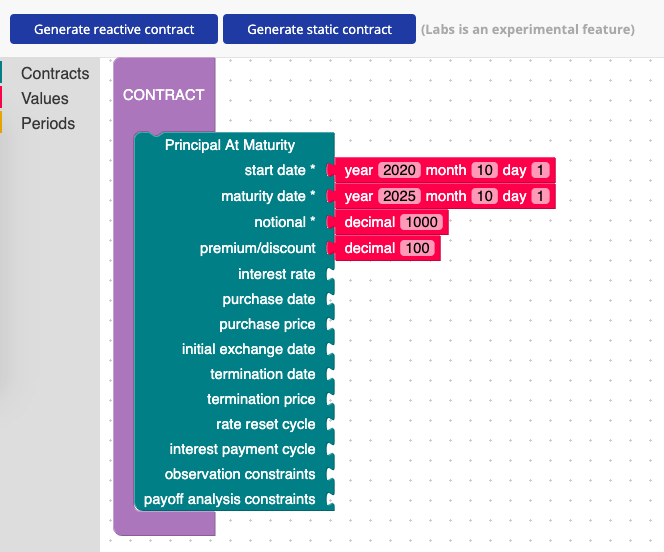
\includegraphics[width=0.8\textwidth]{images/labs.png}
\caption{Actus Labs - an online tool for generating Actus contracts for Marlowe.} 
\label{fig3} 
\end{figure} 

In order to demonstrate and test the capabilities of Actus generators,
a visual online Blockly-based tool was developed for the Marlowe Playground.
The Actus Labs tool, shown in Figure \ref{fig3}, allows users to construct contract terms visually
to generate a corresponding Marlowe contract and then to try it out in a simulation 
environment.

\section{Tokenization}
\label{tokenization}

Every participant of a Marlowe contact %ACTUS contract 
is described by a \texttt{Role} which
is in its turn represented through a unique non-fungible token, created at the time that the contract instantiated on the blockchain.
This makes every ACTUS contract a tradable security, allowing a
participant to sell its \emph{share} in a contract by selling a corresponding
role token.

Role tokens can potentially allow more complex manipulation over such shares,
especially when the share represents an incoming cash flow; in that case, participants
send funds to a party represented by a given token. Such a token
would represent a positive cashflow, which in turn could not only become
tradable but could also allow the derivation of tokens representing \emph{fractional parts}
of a particular cash flow in a contract.

Moreover, this process turns ACTUS loans into derivatives. For example, contracts
like \emph{Interest Rate Swap} (and \emph{Swaps} in general) could be approximated
by an \emph{Atomic Swap} of tokens representing incoming cash flows from
loans. 
For example, if Alice has fixed income from a loan, or some other
investment, and Bob has comparable but variable (fluctuating) income,
Bob can hedge by swapping cash flows with Alice. If Alice's income
is locked with \texttt{token1} and Bob's income is locked with \texttt{token2} then an
atomic swap of those tokens is equivalent to a swap of cash flows.

\section{Assurance}
\label{assurance}

We provide assurance to users of our Marlowe ACTUS contracts in a number of ways, as described here. 

\subsection{QuickCheck for cross-testing}

First, we are able to test the executable Haskell implementation
of ACTUS for smart-contracts by comparing it with an existing implementation written in Java. To do this  
%original Java implementation for analytics - 
a simple property-based test in QuickCheck~\cite{qc} was introduced, where we generate contract terms and risk factors randomly to test the property.

\newcommand{\rf}{\ident{rf}}
\newcommand{\ct}{\ident{ct}}
\smallskip
\noindent 
\begin{equation*}
\forall \ct.\forall \rf. \; \ident{getCashFlows}(\ident{"haskell"},\ct,\rf)\equiv \ident{getCashFlows}(\ident{"java"},\ct,\rf)
\end{equation*}
\noindent
where \emph{ct} represents contract terms, \emph{rf} is risk factor model, and
\emph{getCashFlows()} returns a set of \emph{(date,payoff)} tuples.

\subsection{QuickCheck for verification}

QuickCheck contract terms generators also allow us to check
other properties of a Marlowe contract. This could be enhanced
with Marlowe's static analysis feature by utilising the \texttt{Assert} operator:

% SJT what language is this written in?
% can we turn it into Haskell? or Java?
% dk14 it's pseudo-code but I'll make it more Haskell-y
\begin{verbatim}
do
let contractTerms = sample(qcgenerator) 
    contract = generateMarloweContract(contractTerms) 
    contractWithAssert = appendAssertion(contract, assertion) 
runStaticAnalysis(contractWithAssert)
\end{verbatim}

While this scenario does not cover all possible contracts, it could guarantee that
property holds for a statistically significant fraction of a contract.

\subsection{Static analysis for verification}
% SJT added this as a separate sub section, as it covers the static analysis work.
% references added.
% dk14. Thanks

Using static analysis for Marlowe~\cite{marlowe-efficient} it is possible fully to check a particular contract instead of using random
sampling. That would allow some refinements: 
\begin{itemize}
\item More balanced sampling: the space of contract terms depends linearly on
the coverage, e.g. if we cover 10\% of all possible contract terms
- we'll cover 10\% of all contracts. Different contracts have different
sets of risk factors, and so different search spaces. For instance, a
contract with 3 risk factors (e.g. 3 observations of an interest rate)
would span over $n^3$ values while a contract with 10 risk
factors would span over $n^{10}$. Meanwhile, the space of
all risk factors in all contracts doesn't linearly depend on the coverage.
% SJT explain last sentence. 
\item Dependency tracking: an SMT-solver is potentially likely to be more aware of execution
paths that lead to the failure of a test, a feature that could significantly reduce
search space. 
\item Completeness: if not timed out, SMT-solving is decidable while sampling
is semi-decidable. 
\end{itemize}

\subsection{Securing collateral logic with auto-refund warnings}

By design, the Marlowe interpreter always refunds any assets held in a
contract when it terminates. This is done in order to ensure that
no funds are lost forever. The funds are returned to whoever's internal
account  holds them.

However, this presents as a problem in certain cases where ownership
of the funds could not be  determined automatically. For example, if
Alice puts collateral in a crypto-loan contract she would formally
maintain ownership, which means she would get automatically refunded
when a \texttt{Close} construct is reached.

This implicit refund is easy to overlook by smart-contract developers
as plain \texttt{Close} is often used as a default action in case of unexpected
behaviour like timeouts, and especially a \texttt{Choice} timeout. This can easily
lead to costly %multi-million dollar 
mistakes if  Alice maliciously decides to
exploit an auto-refund feature in order to get her collateral without
paying back, as in the following scenario:
\begin{enumerate}
\item Alice creates a contract where a \texttt{Deposit} timeout would lead to \texttt{Close} 
\item Bob doesn't know or test the timeout path. Even if Bob is a programmer,
he might not be aware that \texttt{Close}ing the contract would cause the collateral
to be refunded to Alice.
\item Alice puts her collateral in the contract and gets the notional from Bob.
\item Alice doesn't pay for the loan: i.e. there is a \texttt{Deposit} timeout. 
\item Alice gets her collateral back. 
\item Bob loses his notional. 
\end{enumerate}
In order to prevent this from happening, an additional \texttt{Auto-Refund}
security check was introduced as part of static analysis tooling which
notifies users about all \texttt{Close} constructs that can lead to automatic
refunds and encourages users to write explicit logic for edge cases.

\section{Related work}\label{related}

% SJT changed title from {Comparison with existing smart-contracts approaches }
% it's traditional to call this "related work".
% dk14. sure this is better


Unlike current popular DeFi lending approaches - Marlowe ACTUS-based
implementation tends to rely on trade-matching instead of pooling.
While asset pooling is proven to be superior to order-book based approaches
when it comes to automated market makers, using it for lending has
been shown to be more susceptible to attacks\cite{flash-loan}.

Moving trade matching off-chain also improves scalability of the protocol
- every loan is a separate contract, thus there is no global state.

Actus provides additional benefit of being regulatory friendly, ACTUS
foundation provides a set of tools allowing Monte-Carlo simulations
of ACTUS contracts.

\section{Conclusion}
\label{conclusion}

Marlowe language was explicitly designed as a set of building blocks
for financial contracts that could be combined by anyone familiar
with basic programming. Marlowe ACTUS generators improve on that by
providing a way to automatically combine blocks based on standardized
requirements specified by the user.

On top of that, Marlowe ACTUS provides a toolkit for cross-testing
with original ACTUS spec, a framework for adding new contract types,
cash-flow visualisations and verification tooling.

%
% ---- Bibliography ----
%
% BibTeX users should specify bibliography style 'splncs04'.
% References will then be sorted and formatted in the correct style.
%
\bibliographystyle{splncs04}
\bibliography{article}
%

\end{document}
